
\documentclass{book}
\usepackage{a4,makeidx,fancyheadings}
\usepackage{graphicx}
\usepackage[francais]{babel}
\usepackage[utf8]{inputenc}
\usepackage{fancyvrb}
\usepackage{makeidx}
\usepackage{tabularx}
\usepackage{eurosym}
\usepackage{color}
\usepackage{url}
\usepackage{geometry}
\geometry{ 
      hmargin=3cm,
      vmargin=3cm
}

\makeindex

%--------------------------------------
%pour compiler avec latex ou pdflatex
\newif\ifpdf
\ifx\pdfoutput\undefined
  \pdffalse
\else
  \pdfoutput=1
  \pdftrue
\fi
%--------------------------------------
	
\begin{document}
\newcommand{\motcle}[1]{\index{#1}\emph{#1}}
\newcommand{\instrcle}[1]{\index{\texttt{#1}}\texttt{#1}}

\thispagestyle{empty}
%-------- fancy headings setting -----------
\rhead[]{}
%\footrulewidth 0.1pt
\rfoot[]{\small\sc S. Genaud}
\pagestyle{fancy}
%------------------------- Page de Garde -------------------
\setlength{\parindent}{0mm}
\setlength{\parskip}{0mm}
\vspace*{\stretch{1}}
\rule{\linewidth}{1mm}
\begin{center}
\Large{Audit du Système d'Information}\\[5mm]
\Large{de l'Ecole de Management de Strasbourg}\\[5mm]
\large{Stéphane Genaud}
\rule{\linewidth}{1mm}
\vspace*{\stretch{2}}
\end{center}
\begin{center}
juin \oldstylenums{2011} \\
\textrm{
$Revision$\\
$Id$\\
$Date$\\
}
\end{center}
%------------------------------------------------------------

\tableofcontents
\newpage

 
 

\chapter{Services Audités}
 

\subsection{Responsable Informatique}

\paragraph{Christos Karakostas} (Responsable)


\subsection{Recherche}
\paragraph{Maxime Merli, Thierry Nobre, Karine Bouvier}

\paragraph{Processus fonctionnels}
Le besoin quasi-exclusif est le recensement des publications des chercheurs.
Cette information sert à deux types processus:
\begin{itemize}
\item L'évaluation de la production scientifique individuelle ou 
collective (AERES, accrédiations, classements, etc).
\item La communication sur les centres d'intérêts et compétences 
vers l'extérieur (sites web, faculty book, etc).
\end{itemize}

L'information doit être structurée de façon à répondre aux exigences des 
différentes instances d'évaluations (AERES, organismes d'accréditation).
Cette structuration des informations bibliographique est classique et des
formats existent depuis longtemps (par exemple bibtex). Une spécificité
à prendre en compte est les classements des revues établi annuellement par 
l'AERES.

D'autres processus peuvent être identifiés, comme par exemple l'organisation
d'une conférence, où la collecte d'information concernant le devenir des
doctorants. Cependant, l'essentiel de ces actions sont ponctuelles et ne 
nécessitent pas un support récurrent du système d'information. La seule 
activité récurrente annexe identifiée est la consultation de l'état des 
finances. Dans ce cas, l'interface web avec SIFAC ainsi que les contacts 
nécessaires avec le gestionnaire des comptes apparaissent satisfaisants.



\paragraph{Existant}
L'existant est essentiellement constitué de:
\begin{itemize}
\item la base de données recherche (MS Access), propre à l'EM,
\item l'application, partie de l'intranet, qui gère cette base : saisie, 
modification, consultation de la base.
\end{itemize}
Un premier projet a été mené en 2010 pour constuire cette base de données des
publications des enseignants-chercheurs de l'EM Strasbourg. Il a été demandé à 
CK de développer une fonctionnalité de l'intranet pour cela. L'interface de 
saisie développée n'étant pas assez contrainte, ce premier projet n'a pas 
permis de collecter des données d'une qualité suffisante pour être exploitables
pour produire les statistiques requises (e.g noms de revues orthographiées 
différement). Sur la base de ce constat, l'outil de collecte a été amélioré en 
2011. Du point de vue des responsables du projet (MM, KB, TN) l'outil donne 
satisfaction en concerne la qualité des données. Des fonctionnalités supplémentaires 
sont envisagées de manière non urgente (fichier PDF téléchargeable de la publication,
remontée automatique du papier sur des archives ouvertes comme SSRN%
\footnote{\url{ http://www.ssrn.com/}}).
La façon dont les informations sont présentées sur les pages web personnelles
des enseignants-chercheurs%
\footnote{\url{http://www.em-strasbourg.eu/enseignants/em-strasbourg-enseignants}}
est également jugé satisfaisant.

\paragraph{Qualité des applications}
Il est à noter que l'interface construite ne permet pas de faire d'import (bibtex, 
endnotes,~...). 


\paragraph{Observations générales}
Il ressort de la discussion que les principaux problèmes auxquels ont eu à 
faire MM et KB pour la mise en place du projet sont:
\begin{itemize}
\item un problème d'interlocuteur : ils n'ont pas trouvé de personne référente 
capable de les orienter sur les ressources internes ou externes, capables de fournir 
la prestation dont ils avaient besoin.
\item un problème de conduite de projet : une fois la ressource chargée de la 
réalisation identifiée (CK), leur demande n'a pas fait l'objet d'une conduite
de projet. La planification était hasardeuse, le cahier des charges et
les validations peu formalisées.
\end{itemize}




\subsection{Relations Externes}
\paragraph{Marie-Hélène Brémont, Hélène Heitz}

\subsection{Service communication}
Michèle Schmidt (MS), Isabelle Suhr (IS), Nicolas Beyhurst (NB),

\paragraph{Processus fonctionnels}
Les processus nécessitant le support du système d'information peuvent 
être rangés en quatre catégories:
\begin{itemize}
\item i) La communication d'informations à des publics ciblés
\item ii) La gestion technique d'évènementiels 
\item iii) La collecte d'informations pour répondre aux enquêtes de type palmarès
\item iv) L'analyse de l'attractivité de chaque formation académique
\end{itemize}
\bigskip

Dans la catégorie i) le besoin est de constuire des listes pertinentes 
et ciblées d'adresses electroniques. Dans les faits, le mailing est
souvent fait de manière indirecte : l'information est communiquée par
le service en charge du public visé. Une invitation à un colloque académique
sera transmise par Karine Bouvier (Recherche) ou une invitation à un
carrefour métier sera transmise par Bernadette Fischbach (Relations Entreprises).\\

Dans la catégorie ii) on trouve en particulier l'activité de création
de mini-sites par NB permettant de gérer chaque évènement (inscriptions,
programmes, informations pratiques, etc) ou du site des diplômés (alumnis).\\


La catégorie iii) nécessite de rassembler des statistiques provenant de 
nombreuses sources. Les informations à collecter et les services qui les 
produisent sont présentés en figure~\ref{fg:comm_flux}.
\begin{figure}[hbt]
\begin{center}
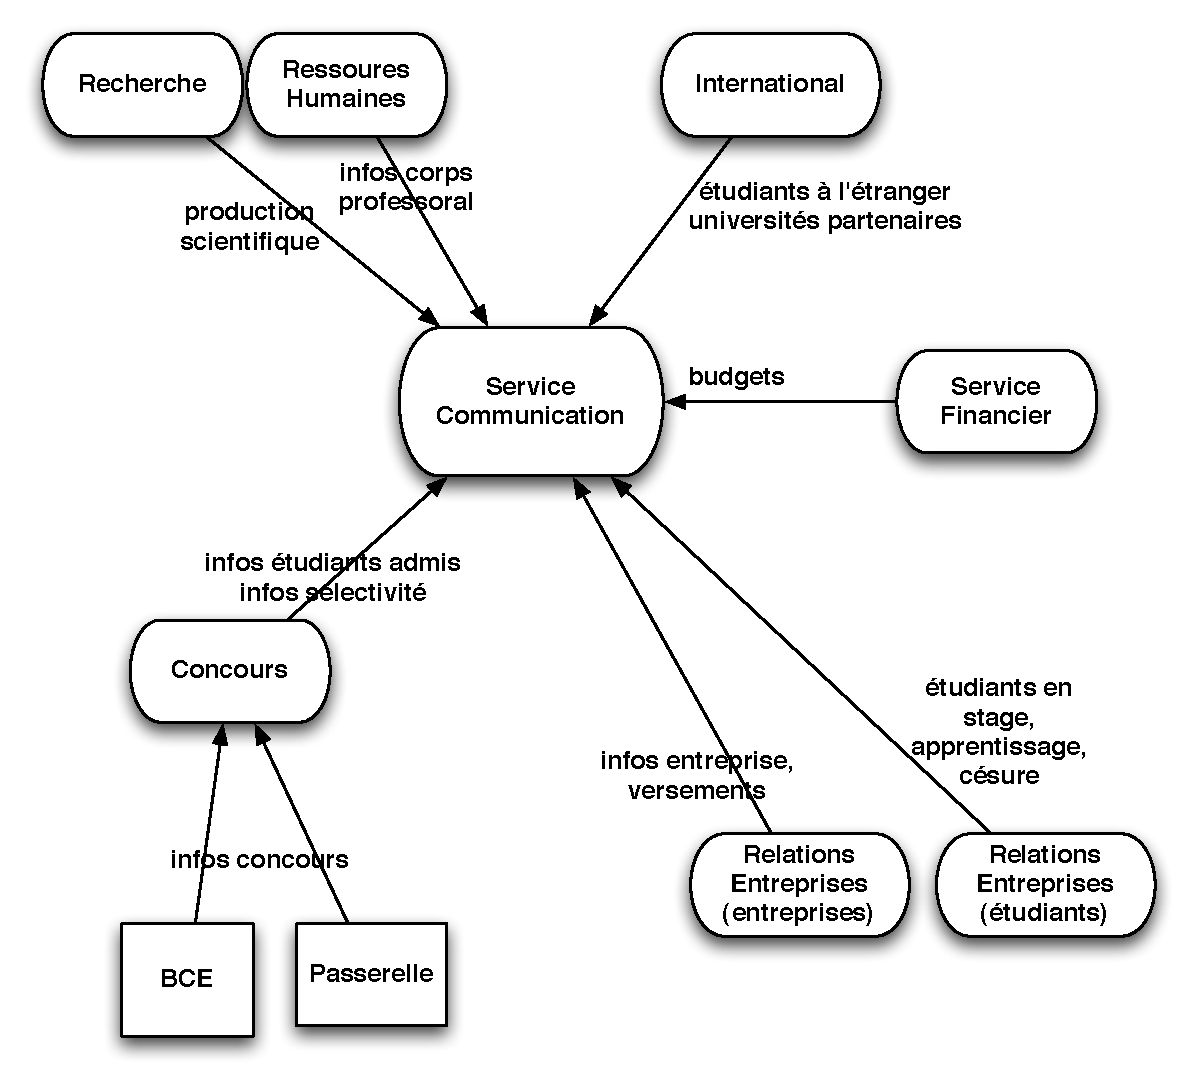
\includegraphics[width=.75\linewidth]{figs/comm_flux.pdf}
\end{center}
\label{fg:comm_flux}
\caption{Les flux d'informations nécessaires pour répondre aux enquêtes}
\end{figure}
Dans ces enquêtes, MS sépare les différentes questions posées et délègue
dans les services appropriés la charge de trouver l'information.\\


La catégorie iv) cible la connaissance  ...


\paragraph{Existant}
\begin{itemize}
\item i) il existe des fichiers prospects dispersés. Ceux-ci ont pu être 
      constitués par la collecte des informations saisies par un participant
      à un évènement (inscription sur mini-site), ou lors de salons (saisie
	manuelle). Lapplication ARIA de pré-candidature peut aussi être utilisée
	pour produire des fichiers prospects (personnes ayant entamé une démarche
	d'inscription sans finaliser).

\item 
\end{itemize}





\subsection{Ressources humaines}
Laurie Walbrou

\subsection{Executive Education }
Pia Imbs (Directrice déléguée)

\subsection{Accréditations}
Maxime Merli, Fatiha Boutera

\subsection{Concours }
Aida Saïd, responsable

\subsection{EM Strasbourg Partenaires }
Francis Schillio, Directeur 

\subsection{Masters Universitaires}
Géraldine Broye (Directrice déléguée),

 
\subsection{Scolarités}

\subsection{Programme Grande Ecole}
Babak Mehmanpazir, (Directeur déléguée)

\subsection{Service International}

\subsection{Université numérique}

%----------------------- BIBLIO ----------------------------------------------
\bibliographystyle{alpha}
\bibliography{biblio}
%----------------------- ANNEXES -------------------------------------
\appendix
%\chapter{Objets - manuel de r�f�rence}	  
\label{ch:annexea}
\newcommand{\n}{\textsf{Netscape$\:$}}
\newcommand{\ie}{\textsf{Internet Explorer$\:$}}
	   
\section{anchor}

   Une ancre (anchor) est un rep�re dans une page. L'utilit� de l'ancre est de pouvoir amener l'utilisateur directement sur la zone de la page marqu�e par ce rep�re. Ceci n'est g�n�ralement utilis� que quand la page est longue.
zone d'une page. An example of an anchor would be
  

\paragraph{Syntaxe}   \verb@<A NAME="mon-ancre">@ 

qui fait r�f�rence � l'ancre d�finie par 
\verb@<A HREF="#mon-ancre">@

\paragraph{Propri�t�s} aucune
\paragraph{M�thodes} aucune
	  
\section{array} 

Les tableaux servent � stocker d'autres objets. 
comme par exemple plusieurs champs dans un formulaire. 
Les diff�rents �l�ments sont rang�s dans un tableau dans l'ordre o� 
ils apparaissent.
 
\paragraph{Propri�t�s}  length
\paragraph{M�thodes}  aucune

%----------------------------------------------------------------------	
\section{button}

 L'objet button ainsi que ses propri�t�s sont d�finis dans un formulaire. 
 La propri�t� value est le texte appara�ssant sur le boutton. 
 
\paragraph{Syntaxe}   \verb@<INPUT TYPE="button" name="Name" value="value">@
\paragraph{Propri�t�s}   name et value
\paragraph{M�thodes}   click()
\paragraph{Ev�nements} onBlur, onClick, onFocus, onMouseDown, onMouseUp 
%----------------------------------------------------------------------	
\section{checkbox} 

Une checkbox a l'apparence d'une bo�te carr�e qu'on s�lectionne ou
d�selectionne par un clic de souris. Les checkbox sont d�finies �
l'aide de la balise \verb@<FORM>@.
    
\paragraph{Syntaxe}   \verb@<INPUT TYPE="checkbox" name="Name" value="value">@
\paragraph{Propri�t�s}   checked, defaultChecked, name, and value
\paragraph{M�thodes}   blur(), click(), focus()
\paragraph{Ev�nements} onBlur, onClick, onFocus 
 
%----------------------------------------------------------------------	
\section{Date} 

L'objet date est un objet dot� de nombreuses m�thodes de manipulation.  
JavaScript m�morise les dates comme le nombre de millisecondes (ms) �coul�es depuis le 1er Janvier 1970.
  
 
\paragraph{Propri�t�s}  aucune
\paragraph{M�thodes} 

\[
\begin{tabular}{ll}
          getDate() & rend le jour du mois de la date courante\\
          getDay() & rend le jour de la semaine de la date courante \\
          getHours() & rend le jour de la semaine de la date courante\\
          getMinutes() & rend les minutes de la date courante\\
          getMonth() & rend le mois de la date courante\\
          getSeconds() & rend les secondes de la date courante\\
          getTime() & rend la valeur num�rique de la date courante\\
          getTimezoneOffset() & rend le d�calage horaire en minutes avec GMT\\
          getYear() & rend l'ann�e de la date courante\\
          parse(d) & rend le nombre de ms �coul�es entre $d$ et le 1/1/70\\
          setDate(j) & met � la jour la date au jour $j$ \\
          setHours(h) & met � la jour la date au jour $h$ \\\\
          setMinutes(m) & met � la jour la date � la minute $m$\\
          setMonth(m) & met � la jour la date au mois $m$\\
          setSeconds(s) & met � la jour la date � la seconde $s$\\
          setTime(n) & met � jour la date �tant donn� le nombre $n$ de ms depuis le 1/1/70\\
          setYear(d) & met � jour l'ann�e pour une date $d$\\
          toGMTString() &  convertit la date une date GMT \\
          toLocaleString() & convertit la date une date locale\\
          UTC(a,m,j) & rend le nombre de ms entre la date et le 1/1/70
\end{tabular}\]
%----------------------------------------------------------------------	
\section{document} 

L'objet document contient les onformations sur le document courant. 
Il fournit aussi des m�thodes pour afficher du texte au format HTML dans le navigateur. 

\paragraph{Propri�t�s}
\[\begin{tabular}[t]{ll}
          alinkColor & couleur d'un lien actif\\
          anchors & tableau regroupant les ancres du document\\
          bgColor & couleur de fond\\
          cookie &  \\
          fgColor & couleur d'avant plan\\
          forms & tableau des formulaires\\
          lastModified & date de deni�re modification\\
          linkColor & couleur des liens\\
          links & tableau des liens\\
          location & URL du document courant\\
          referrer & URL de la page pr�c�demment visit�e\\
          title & titre de la page\\
          vlinkColor & couleur d'un lien visit�\\
\end{tabular}\]

\paragraph{M�thodes} 
\[\begin{tabular}[t]{ll}
	close()	& ferme un flux ouvert par la m�thode open()		\\
	getSelection()	& rend la chaine selectionn�e dans le document courant\\
	open()	& ouvre un flux pour affichage de texte avec write() \\
	write($e_1, .. ,e_n$)& affiche les expressions $e_1,..,e_n$ dans le document.		\\
	writeln($e_1, .. , e_n$) & idem mais ajoute un retour � la ligne\\
\end{tabular}
\]
               
%----------------------------------------------------------------------	
\section{form} 

L'objet form permet de cr�er un formulaire. 
Les formulaires peuvent contenir des champs, des zones de texte des boutons, des checkboxes, etc.  

\paragraph{Syntaxe}

\begin{verbatim}
<FORM NAME="name" TARGET="target" ACTION="file" 
 METHOD="POST/GET" ENCTYPE="encodingtype">
\end{verbatim}
 
o� \verb@TARGET@ d�signe la fen�tre dans laquelle les r�sultats doivent aller,
\verb@ACTION@ d�fini quelle action doit �tre entreprise quand le formulaire � �t� rempli. Ce peut �tre entre autres un nom de fichier HTML � afficher, un script cgi � ex�cuter, ou une adresse electronique vers laquelle envoyer un courrier.
\verb@METHOD@ peut prendre les valeurs POST ou GET, qui d�finissent comment la r�ponse est envoy�e au serveur. \verb@ENCTYPE@ indique l'encodage MIME � utiliser dans le transfert.

\paragraph{Propri�t�s}  action, elements, encoding, length, method, target,
          button, checkbox, hidden, password, radio, reset, select, submit,
          text, et textarea
\paragraph{M�thodes}  submit()
%----------------------------------------------------------------------	
\section{frame}

          L'objet frame permet de manipuler les cadres. 
          Un cadre est une division de la page web en plusieurs zone.
          La balise \texttt{<FRAMESET>} permet de diviser une zone en deux, chacune des zones pouvant �tre nouveau divis�e en deux. 

\paragraph{Syntaxe}
\begin{verbatim}
          <FRAMESET ROWS="x1,x2" COLS="y1,y2">
          <FRAME SRC="file" NAME="name">
          </FRAMESET>
\end{verbatim}
\texttt{ROWS} sp�cifie les nombres de lignes dans le premier cadre
et le deuxi�me cadre par \texttt{x1} et \texttt{x2} respectivement, qui sont
soient des entiers, soit des pourcentages de la zone divis�e.
De la m�me mani�re, \texttt{COLS} sp�cifie la largeur des cadres.
\texttt{SRC} indique quel fichier doit �tre charg� dans le cadre.
 
\paragraph{Propri�t�s} 

\begin{tabular}[t]{ll}
          frames &  \\
          name &  \\
          length &  \\
          parent &  \\
          self &  \\
          window &  \\
\end{tabular}

\paragraph{M�thodes}  clearTimeout(), et setTimeout()
%----------------------------------------------------------------------	
\section{hidden}

L'objet hidden est un champ texte invisible pour l'utilisateur, permettant d'ajouter des informations pr�-d�finies dans un formulaire. 

\paragraph{Syntaxe}

\verb@<INPUT TYPE="hidden" NAME="name" VALUE="value">@
o� \verb@VALUE@ est la valeur du champ.

\paragraph{Propri�t�s}  name et value
\paragraph{M�thodes} : aucune
%----------------------------------------------------------------------	
\section{history} 

L'objet history contient des informations sur la session de navigation en cours.
Les informations sont essentiellement les URL des sites visit�s.
 
\paragraph{Propri�t�s}  length
\paragraph{M�thodes} back(), forward(), et go()
%----------------------------------------------------------------------	
\section{Image} 

L'objet Image contient les informations concernant les images et cartes ins�r�es
dans le document HTML � l'aide des balises \verb@<IMG>@ et \verb@<AREA>@. Les propri�t�s sont disponibles pour \n 3, \n 4 et \ie 4 � l'exception des propri�t�s x et y uniquement disponibles dans \n 4.

\paragraph{Propri�t�s}  
\begin{tabular}[t]{ll}
          border & valeur de l'attribut de m�me nom dans la balise \verb@<IMG>@	\\
          complete & bool�en indiquant si l'image est compl�tement affich�e  \\
          height &  la hauteur de l'image en pixels \\
          hspace &  valeur de l'attribut de m�me nom dans la balise \verb@<IMG>@\\
          lowsrc &  similaire � src, mais pour des images longues � charger\\
          name	& valeur de l'attribut de m�me nom dans la balise \verb@<IMG>@  \\
          src & le nom du fichier image		 \\
          vspace & valeur de l'attribut de m�me nom dans la balise \verb@<IMG>@   \\
          width & valeur de l'attribut de m�me nom dans la balise \verb@<IMG>@	\\
	  x & l'abscisse du coin haut-gauche de l'image	\\
	  y & l'ordonn�e du coin haut-gauche de l'image 	 \\	
\end{tabular} 

\paragraph{M�thodes} aucune 

%----------------------------------------------------------------------		  
\section{link}
 
\paragraph{Syntaxe}

\verb@<HREF="location" NAME="name" TARGET="target">@ avec \verb@HREF@
          l'URL du fichier � charger quand on clique sur le lien, 
	et \verb@TARGET@ est le nom de la fen�tre ou l'afficher.  

\paragraph{Propri�t�s} 
\begin{tabular}[t]{ll}
          hash & ancre dans l'URL\\
          host & nom du serveur dans l'URL\\
          hostname &  adresse IP du serveur\\
          href &  URL compl�te\\
          pathname & texte apr�s le symbole / dans l'URL\\
          port &  port que le serveur utilise\\
          protocol & d�but de l'URL (http,ftp,...)\\
          search & texte apr�s le symbole ? dans l'URL\\
          target & o� afficher la page de cette URL\\
\end{tabular}
\paragraph{M�thodes}  aucune
%----------------------------------------------------------------------	
\section{location}

L'objet location contient les informations sur l'URL courante.

\paragraph{Propri�t�s}  
 \begin{tabular}[t]{ll}
          hash & ancre dans l'URL\\
          host & nom du serveur dans l'URL\\
          hostname &  adresse IP du serveur\\
          href &  URL compl�te\\
          pathname & texte apr�s le symbole / dans l'URL\\
          port &  port que le serveur utilise\\
          protocol & d�but de l'URL (http,ftp,...)\\
          search & texte apr�s le symbole ? dans l'URL\\
          target & o� afficher la page de cette URL\\
\end{tabular}
\paragraph{M�thodes} aucune
%----------------------------------------------------------------------		  
\section{Math}

\paragraph{Propri�t�s} 
\begin{tabular}[t]{ll}
          \verb@E@ &  constante d'Euler ($\sim 2.718$)\\
          \verb@LN2@ &  logarithme de 2 ($\sim  0.693$)\\
          \verb@LN10@ & logarithme de 10 ($\sim2.302$)\\
          \verb@LOG2E@ & Returns the base 2 logarithm of e, about 1.442\\
          \verb@LOG10E@ & Returns the base 10 logarithm of e, about 0.434\\
          \verb@PI@ & valeur de Pi ($\sim 3.14159$)\\
          \verb@SQRT1_2@ &  racine carr�e de $\frac{1}{2}$ ($\sim 0.707$)\\
          \verb@SQRT2@ & racine carr�e de 2 ($\sim 1.414$)\\
\end{tabular}
\paragraph{M�thodes}  

\begin{tabular}[t]{ll}
          abs(x) & rend la valeur absolue de $x$\\ 
          acos(x) & rends arc cosinus de $x$\\ 
          asin(x) & rends arc sinus de $x$\\ 
          atan(x) & rend  l'arc tangente de $x$\\ 
          ceil(x) & rend l'entier imm�diatement sup�rieur ou �gal � $x$\\ 
          cos(x) & rend le cosinus de $x$\\ 
          exp(x) & rend $e^x$\\ 
          floor(x) & rend l'entier imm�diatement inf�rieur ou �gal � $x$\\ 
          log(x) & rend le logarithme de $x$\\ 
          max(x,y) & rend le maximum de $x$ et $y$\\ 
          min(x,y) & rend le minium de $x$ et $y$\\ 
          pow(x,y) & rend $x^y$\\ 
          random() & rend un nombre al�atoire entre 0 et 1\\ 
          round(x) & rend l'entier le plus proche de $x$ \\
          sin(x) & rend le sinus de $x$\\
          sqrt(x) & rend $\sqrt{x}$\\
          tan(x) & rend la tangente de $x$\\
\end{tabular}

\section{navigator} 

 Cet objet permet d'obtenir des informations sur le navigateur visitant la page.
 
\paragraph{Propri�t�s}
\begin{tabular}[t]{ll}
          appCodeName & rend le nom de code du navigateur (Mozilla)\\
          appName & rend le nom commercial du navigateur\\
          appVersion & rend le num�ro de version du navigateur\\
          userAgent & rend le nom complet du navigateur\\
\end{tabular}
\paragraph{M�thodes} aucune
%----------------------------------------------------------------------	  
\section{password}

L'objet password cr�� un champ texte comme l'objet text, mais les caract�res
saisis apparaissent comme des ast�risques, rendant la saise confidentielle
aux yeux d'autres personnes que l'utilisateur. 

\paragraph{Syntaxe}
\begin{verbatim}
         <INPUT TYPE="PASSWORD" NAME="NAME" VALUE="VALUE" SIZE="SIZE">
\end{verbatim}
 
 \texttt{SIZE}  est la largeurdu champ en nombre de caract�res.
    
\paragraph{Propri�t�s} 
\begin{tabular}[t]{ll}
          defaultValue & valeur initiale du champ\\
          name & nom du champ\\
          value & valeur courante du champ\\
\end{tabular}
\paragraph{M�thodes} 
\begin{tabular}[t]{ll}
          blur() &  Enl�ve le curseur du champ\\
          focus() &  Am�ne le curseur dans le champ\\
          select() & S�lectionne le texte saisi\\
\end{tabular}
%----------------------------------------------------------------------	
\section{radio}
 
Les objets radios sont des boutons ne permettant a l'utilisateur de ne choisir 
qu'une option parmi plusieurs.

\paragraph{Syntaxe}  

\verb@<INPUT TYPE="radio" NAME="Name" VALUE="Value" {CHECKED}>@
      
o� \verb@VALUE@ est le texte apparaissant sur le bouton.
En sp�cifiant l'attribut \texttt{CHECKED} alors le bouton est pr�-s�lectionn�
au chargement du formulaire. 

 \paragraph{Propri�t�s} 
\begin{tabular}[t]{ll}
          checked & indique si le bouton � �t� s�lectionn�\\ 
          defaultChecked & indique quel bouton doit �tre pr�-selectionn� \\
          length & donne le nombre de  boutons \\
          object &\\
          name  & permet de donner un nom au(x) bouton(s) \\
          value &  permet de donner une valeur au(x) bouton(s)\\
\end{tabular}
\paragraph{M�thodes}  click()
\paragraph{Ev�nements} onBlur, onClick, onFocus 

%----------------------------------------------------------------------	
\section{reset}

Le bouton reset permet de r�initialiser un formulaire.
 
\paragraph{Syntaxe}

\verb@<INPUT TYPE="RESET" NAME="NAME" VALUE="VALUE">@
o� \verb@VALUE@ est le texte apparaissant sur le bouton.
 
\paragraph{Propri�t�s} 
\begin{tabular}[t]{ll}
          name & Le nom du bouton\\
          value & La chaine associ�e au bouton\\
\end{tabular}

\paragraph{M�thodes}  click()
\paragraph{Ev�nements} onBlur, onClick, onFocus 

%----------------------------------------------------------------------	
\section{select}
\paragraph{Syntaxe}
\begin{verbatim}
          <SELECT NAME="NAME" SIZE="SIZE" {MULTIPLE}> 
          <OPTION VALUE="option"> Texte </SELECT>
\end{verbatim}
o� \texttt{SIZE} fixe le nombre d'options avant de d�rouler le menu (d�faut 1), \texttt{MULTIPLE}, s'il est pr�cis� fait du menu une liste � choix multiple.
L'attribut \verb@<OPTION VALUE="option">@ ajoute une option de menu � chaque fois qu'il est ajout�. Il faut donc un attribut \verb@OPTION@ pour chaque option du menu. 
 
\paragraph{Propri�t�s} 

\begin{tabular}{ll}
          length & Met � jour le nombre d'options	\\
          name &  Met � jour le nom du menu	\\
          options & Tableau des diff�rentes options du menu\\
          selectedIndex & Rend le num�ro de l'option choisie\\
	  \end{tabular}
\paragraph{M�thodes} : blur(), et focus()
\paragraph{Ev�nements} onBlur, onChange, onFocus 

%----------------------------------------------------------------------	
\section{string}
\label{sc:appendix-string}
\paragraph{Propri�t�s}  length
\paragraph{M�thodes} 

\begin{tabular}[t]{ll}
          big & Affiche la chaine dans une grande police\\
          blink & Affiche la chaine en clignotant\\
          bold & Affiche la chaine en caract�res gras\\
          charAt & Rend le caract�re � une certaine position dans la chaine\\
          fixed & Affiche la chaine dans une police � taille fixe\\
          fontcolor & La couleur de fond d'affichage de la chaine\\
          fontsize & La taille de la police d'affichage de la chaine\\
          indexOf & Rend la premi�re occurence d'une sous-chaine dans la chaine\\
          italics & Affiche la chaine en italique\\
          lastIndexOf & Cherche la derni�re occurence d'une valeur dans une chaine\\
          link & affiche La chaine comme un lien\\
          small & Affiche la chaine en petite police\\
          strike & Affiche la chaine avec une barre en travers\\
          sub & Affiche la chaine en mode indice (subscript)\\
          substring & R�f�rence une sous-chaine\\
          sup & Affiche la chaine en mode exposant (superscript)\\
          toLowerCase & Change la chaine en minuscules\\
          toUpperCase & Change la chaine en majuscules \\
\end{tabular}
%----------------------------------------------------------------------	
\section{submit} 

L'objet submit est le bouton permettant de valider un formulaire. 

\paragraph{Syntaxe}
          
\verb@<INPUT TYPE="SUBMIT" NAME="NAME" VALUE="Text">@ o� VALUE est le texte
affich� sur le bouton.

\paragraph{Propri�t�s}  name, et value
\paragraph{M�thodes} click()
\paragraph{Ev�nements} onClick   

              
%----------------------------------------------------------------------	
\section{text}

 Un objet text est un champ de saisie sur une ligne permettant de saisir toute chaine alphanum�rique. 
 
\paragraph{Syntaxe}

\verb@<INPUT TYPE="text" NAME="name" VALUE="value" SIZE="size">@
o� \texttt{VALUE} est le texte affich� initialement dans le champ, et
\texttt{SIZE} est la largeur du champ en nombre de caract�res.
 
\paragraph{Propri�t�s} defaultValue, name, form, type, value
\paragraph{M�thodes}  focus, blur, and select
\paragraph{Ev�nements} onBlur, onChange, onFocus, onSelect  

%----------------------------------------------------------------------	
\section{textarea} 

L'objet textarea permet � l'utilisateur de saisir plusieurs lignes de
textes dans un formulaire.
 
\paragraph{Syntaxe}

\begin{verbatim}
            <TEXTAREA NAME="name" ROWS=rows COLS=cols
             WRAP="off/virtual/physical">Text</TEXTAREA>
\end{verbatim}
o� \texttt{rows} sp�cifie le nombre de lignes du champ, et \texttt{cols} le nombre de caract�res par ligne.  

\paragraph{Propri�t�s}   defaultValue, name, et select
\paragraph{M�thodes}   focus, blur, et select
\paragraph{Ev�nements} onBlur, onChange, onFocus, onKeyDown, onKeyPress, onKeyUp, onSelect  
%----------------------------------------------------------------------	
\section{window} 
 
\paragraph{Syntaxe}
	\verb@w = window.open("URL", "NAME" {,"Options"})@.\\

o� \verb@URL@ est l'adresse de la page � ouvrir, 
\verb@NAME@ est le nom de la fen�tre, 
et Options sont des param�tres optionels comme la taille de la fen�tre, etc.\\
  
\paragraph{Propri�t�s} 
\begin{tabular}[t]{ll}
          defaultStatus & Le message affich� par d�faut dans la barre de statut\\
          document & Permet d'acc�der au document courant\\
          frames &  Le tableau contenant les cadres de la fen�tre\\
          frame & La fen\^{e}tre avec ascenseur utilis�e pour un tableau\\
          length & Le nombre de cadre dans la fen�tre\\
          location & L'URL du document courant\\
          name & Le nom de la fen�tre\\
          parent & La fen�tre englobante\\
          self & R�f�rence � la fen�tre elle-m�me\\
          status & Le message de la barre de statut\\
          top & R�f�rence � la fen�tre m�re\\
          window & R�f�rence � la fen�tre courante\\
\end{tabular}
\paragraph{M�thodes}
\begin{tabular}[t]{ll}
          alert() 	& Cr�� une boite de dialogue de type message+OK	\\
          close() 	& Ferme le document	\\
          confirm() 	& Cr�� une boite de dialogue de type message+OK/Cancel\\
          open() 	& Ouvre une nouvelle fen�tre \\
          prompt() 	& Cr�� une boite de dialogue de type message+zone de
	  saisie+OK/Cancel\\
          setTimeout() 	&  Ex�cute le code JavaScript apr�s un certain nombre de
	  millisecondes\\
          clearTimeout() & Annule l'effet de la commande setTimeout()\\
\end{tabular} 
%----------------------------------------------------------------------	

\printindex
\end{document}

 

  
 

